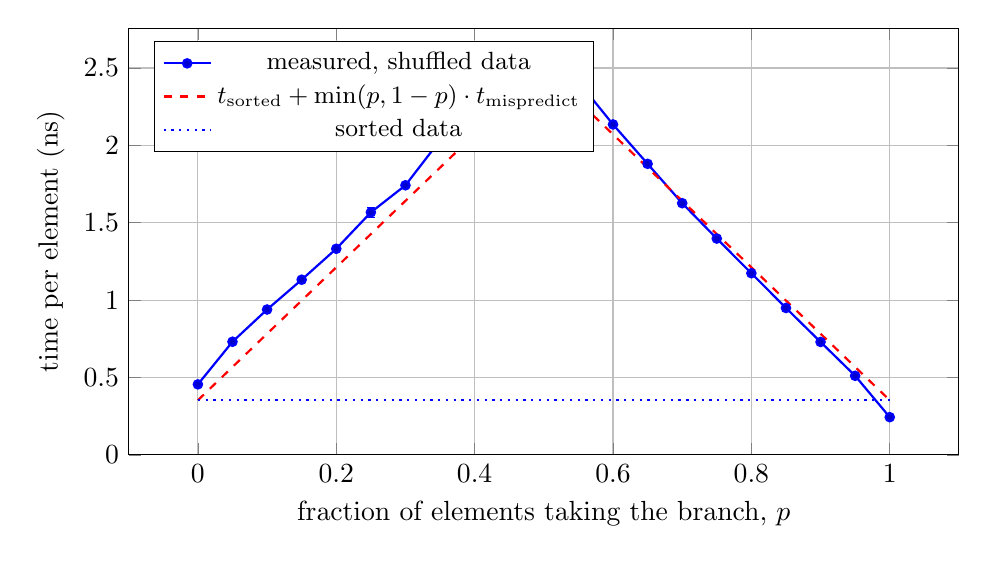
\begin{tikzpicture}
\begin{axis}[width=\textwidth, height=7cm, xlabel={fraction of elements taking the branch, $p$}, ylabel={time per element (ns)}, grid=major, ymin=0,
  legend pos=north west, legend style={font=\small}]
\addplot+[mark=*, mark size=1.5pt, thick, error bars/.cd, y dir=both, y explicit] coordinates {(0.0,0.4556) +- (0,0.003) (0.05,0.731) +- (0,0.002) (0.1,0.9392) +- (0,0.004) (0.15,1.1318) +- (0,0.002) (0.2,1.3317) +- (0,0.004) (0.25,1.567) +- (0,0.031) (0.3,1.742) +- (0,0.002) (0.35,2.0323) +- (0,0.050) (0.4,2.2132) +- (0,0.009) (0.45,2.4286) +- (0,0.007) (0.5,2.5002) +- (0,0.006) (0.55,2.4114) +- (0,0.042) (0.6,2.1352) +- (0,0.011) (0.65,1.8805) +- (0,0.016) (0.7,1.6262) +- (0,0.007) (0.75,1.3976) +- (0,0.005) (0.8,1.1737) +- (0,0.002) (0.85,0.9492) +- (0,0.003) (0.9,0.7295) +- (0,0.004) (0.95,0.5109) +- (0,0.003) (1.0,0.2436) +- (0,0.003)};
\addlegendentry{measured, shuffled data}
\addplot[red, dashed, thick, domain=0:1, samples=101] {0.3531 + min(x,1-x)*4.2942};
\addlegendentry{$t_{\mathrm{sorted}} + \min(p,1-p)\cdot t_{\mathrm{mispredict}}$}
\addplot[blue, dotted, thick, domain=0:1] {0.3531};
\addlegendentry{sorted data}
\end{axis}
\end{tikzpicture}